\documentclass[conference]{IEEEtran}
\IEEEoverridecommandlockouts
% The preceding line is only needed to identify funding in the first footnote. If that is unneeded, please comment it out.
\usepackage{cite}
\usepackage{amsmath,amssymb,amsfonts}
\usepackage{algorithmic}
\usepackage{graphicx}
\usepackage{textcomp}
\usepackage{xcolor}
\def\BibTeX{{\rm B\kern-.05em{\sc i\kern-.025em b}\kern-.08em
    T\kern-.1667em\lower.7ex\hbox{E}\kern-.125emX}}
\begin{document}

\title{Estatísticas de preços de automóveis de passeio - AutoStats\\
\thanks{}
}

\author{\IEEEauthorblockN{Artur P. Carneiro}
\IEEEauthorblockA{\textit{Dept. De Inteligência Artificial Aplicada à Robótica} \\
\textit{FEI - Fundação Educacional Inaciana}\\
São Bernardo do Campo, Brasil \\
acarneiro@fei.edu.br}
}

\maketitle

\begin{abstract}
Esse artigo sintetiza o protótipo de uma solução para pesquisa estatística sobre os valores dos automóveis de passeio (novos e usados) no Brasil.

Esse protótipo é a resposta à um trabalho de conclusão do curso da disciplina de Ciência de Dados, ministrada para os alunos de pós-graduação dos cursos de Mestrado e Doutorado da FEI - Fundação Educacional Inaciana.
\end{abstract}

\begin{IEEEkeywords}
ciência de dados, automóveis de passeio, valor, estatística
\end{IEEEkeywords}

\section{Introdução}
Explicar ou equacionar a evolução dos preços de veículos automotores de passeio (também chamados de carros) no mercado brasileiro, usados ou novos, tem se mostrado um verdadeiro desafio para o comprador. Semelhante desafio é planejar o momento de venda/troca do veículo ou estimar o valor de compra/venda deste. Os fatores que influenciam nos valores dos carros novos vão desde questões produtivas (como a queda da oferta de componentes eletrônicos durante a pandemia do Corona Vírus) até questões econômicas (como a entrada de novos \textit{players} `agressivos', com preços menores para carros mais tecnológicos, ou a redução temporária de impostos pelo governo federal), passando por ações protecionistas dos fabricantes de veículos que optam por parar de produzir e manter os estoques cheios à baixar a margem de lucro por unidade e ganhar na escala, aumentando a produção e esvaziando os estoques. Enquanto isso, o valor dos carros usados é impactado, principalmente, pela capacidade de compra do carro novo pela população, fazendo os preços dos carros usados aumentarem quando a quantidade de novos vendidos diminui e vice-versa. 

Toda essa dinâmica complexa impacta na tomada de decisão por parte do comprador/vendedor, que deve decidir, além do valor inicial da compra (à vista ou financiada) do veículo, questões como custos de seguro, manutenção, documentação e desvalorização do veículo até o momento de "revenda" futuro.

Auxiliar o comprador/vendedor nesta tarefa de análise e tomada de decisão é a motivação da solução proposta pelo protótipo aqui apresentado.

A solução aqui descrita propõe coletar dados sobre a evolução de preços dos veículos em outros sistemas independentes (Fundação Instituto de Pesquisas Econômicas - Fipe, OLX e WebMortors) e indicadores econômicos (Índice Nacional de Preços ao Consumidor Amplo - IPCA, Índice Nacional de Preços ao Consumidor - INPC, Índice de Preços ao Consumidor - IPC-Fipe e o Índice Geral Preços - IGP-M ), concentrá-los e organizá-los para apresentar ao usuário gráficos e informações que sirvam de insumos para a análise de tomada de decisão quanto à compra/venda de um veículo.

O Desenvolvimento é orientado às etapas do ciclo dos dados:

\begin{itemize}
	\item Geração
	\item Coleta
	\item Processamento
	\item Armazenamento
	\item Gerenciamento
	\item Análise
	\item Visualização
	\item Interpretação
\end{itemize}

Por tratar-se de um protótipo que visa demonstrar a viabilidade da solução, os dados são limitados à posteriores a janeiro de 2013 e as informações produzidas se restringem a modelos da marca Volkswagen onde, dado um modelo de veículo específico, são gerados gráficos comparativos da evolução do valor de em relação aos índices de preço, percentual de desvalorização mensal e evolução do preço deste modelo novo (zero quilômetro).

\section{Geração}

\subsection{Preço dos veículos de passeio }

Como fonte de informação sobre preços de veículos de passeio novos e usados, utiliza-se três origens distintas. A primeira refere-se à origem oficial do preço médio de veículos de passeio com valores  reconhecidos por instituições financeiras como a referência de valor dos veículos, utilizados em contratos e decisões judiciais. Esses valores são disponibilizados em consulta gratuita pela Fipe \cite{Fipe}, na página https://veiculos.fipe.org.br/.  

As outras fontes de informações são sites de vendas (WebMotors e OLX), que concentram anúncios de diversos lojistas e/ou pessoas físicas interessadas em vender seus veículos. O WebMotors é um \textit{"marketplace"} exclusivamente de veículos novos ou usados. O OLX, por sua vez, possui uma variedade de produtos, mas é muito utilizado por pessoas interessadas em vender carros usados também.

\subsection{Indicadores Econômicos}

O portal Debit \cite{Debit} disponibiliza em  `https://debit.com.br/tabelas/ipca-indice-nacional-de-precos-ao-consumidor-amplo.php' uma tabela com a variação mensal do IPCA desde 1980. Esses valores são fornecidos pelo IBGE \cite{IBGE}, mensalmente.

Esta mesma solução disponibiliza a tabela do Índice Geral de Preços Médios (IGP-M), produzido pela Fundação Getúlio Vargas - FGV \cite{FGV}, desde 1989 em 'https://debit.com.br/tabelas/tabela-completa.php?indice=igpm´.

O portal da Fipe disponibiliza as taxas mensais do Índice de Preços ao Consumidor - IPC, desde 2011, em 'https://www.fipe.org.br/pt-br/indices/ipc/\#indice-mensal´.


\section{Coleta}

\subsection{Preço médio de veículos de passeio - Fipe}

A solução da Fipe utiliza de serviços para carregar as informações dinamicamente na página (o que chamamos de AJAX) e realizar as consultas (serviços disponibilizados em 'https://veiculos.fipe.org.br/api/veiculos´). Esses serviços não são controlados ou autenticados. Isso possibilita executar um processo de captura dos dados consumindo diretamente os serviços. São eles:

\begin{itemize}
	\item 'ConsultarTabelaDeReferencia´: retorna uma lista de referências (mês/ano) possíveis. Compreende ao mês e o ano da coleta dos preços médios dos veículos.
	\item 'ConsultarMarcas´: retorna as marcas presentes uma dada referência.
	\item 'ConsultarModelos´: retorna os modelos existentes nos resultados, dado a marca e referência.
	\item 'ConsultarAnoModelo´ : retorna os anos de fabricação existentes, dado o modelo, marca e referência.
	\item 'ConsultarValorComTodosParametros´ : retorna o valor de um veículo dado um ano de fabricação, modelo, marca e referência. 
\end{itemize}

O protótipo, então, realiza a coleta dos dados de preços por um \textit{'script´ Python}, total ou parcial, atualizando esses dados no banco de dados utilizado na aplicação.


\subsection{Preço médio "Real" de venda em estabelecimentos comerciais}

Os \textit{marketplaces} WebMotors e OLX foram desenvolvidos de maneira à não permitir que requisições não vindas de seus próprios \textit{sites} acessem os serviços "AJAX". Desta forma, não é possível utilizar a mesma estratégia de coleta utilizada no portal da Fipe.

Nestes casos utiliza-se da estratégia chamada \textit{'web crawler´} onde um \textit{script} Python realiza uma 'navegação sistêmica´ aos portais e captura as informações geradas, passando-se por um usuário humano. 

Para OLX, faz-se uma requisição ao endereço:

https://www.olx.com.br/brasil?q=\{FABRICANTE\} \{MODELO\} \{ANO\}


\begin{figure}[h!]
	\centerline{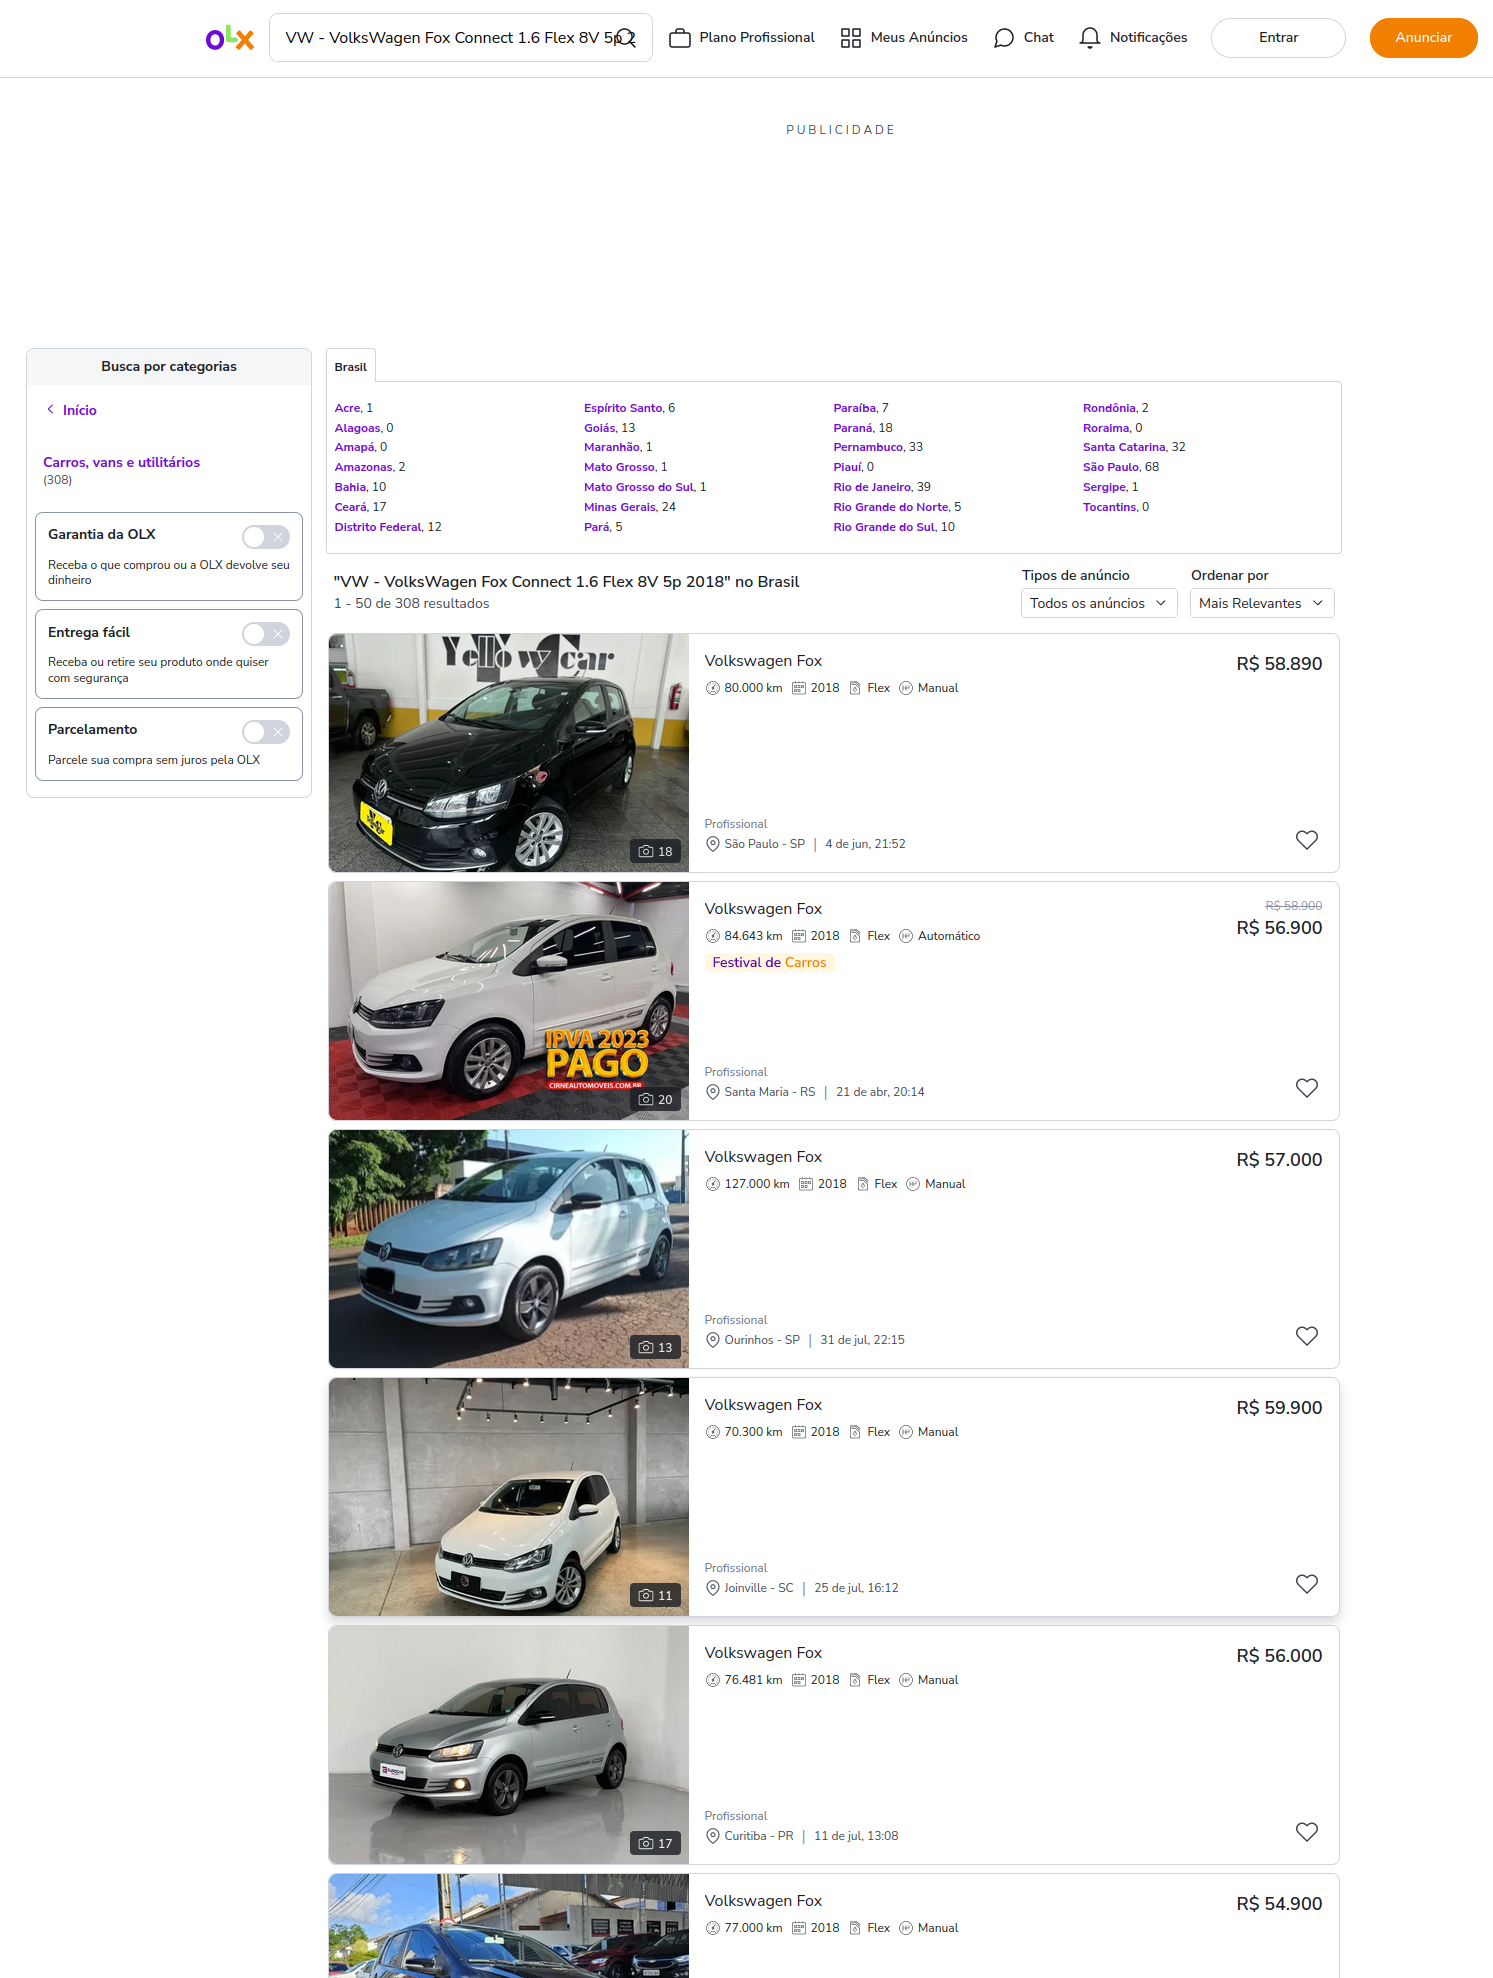
\includegraphics[width=250pt]{assets/olx.png}}
	\caption{Site de anúncios da OLX.}
	\label{fig5}
\end{figure}

Para o WebMotors, navega-se em:

https://www.webmotors.com.br/carros?tipoveiculo=carros\& anoate=\{ANO\}\&anode=\{ANO\}\&marca1=\{FABRICANTE\}\& modelo1=\{MODELO\}\&versao1=\{VERSÃO DO MODELO\}


\begin{figure}[h!]
	\centerline{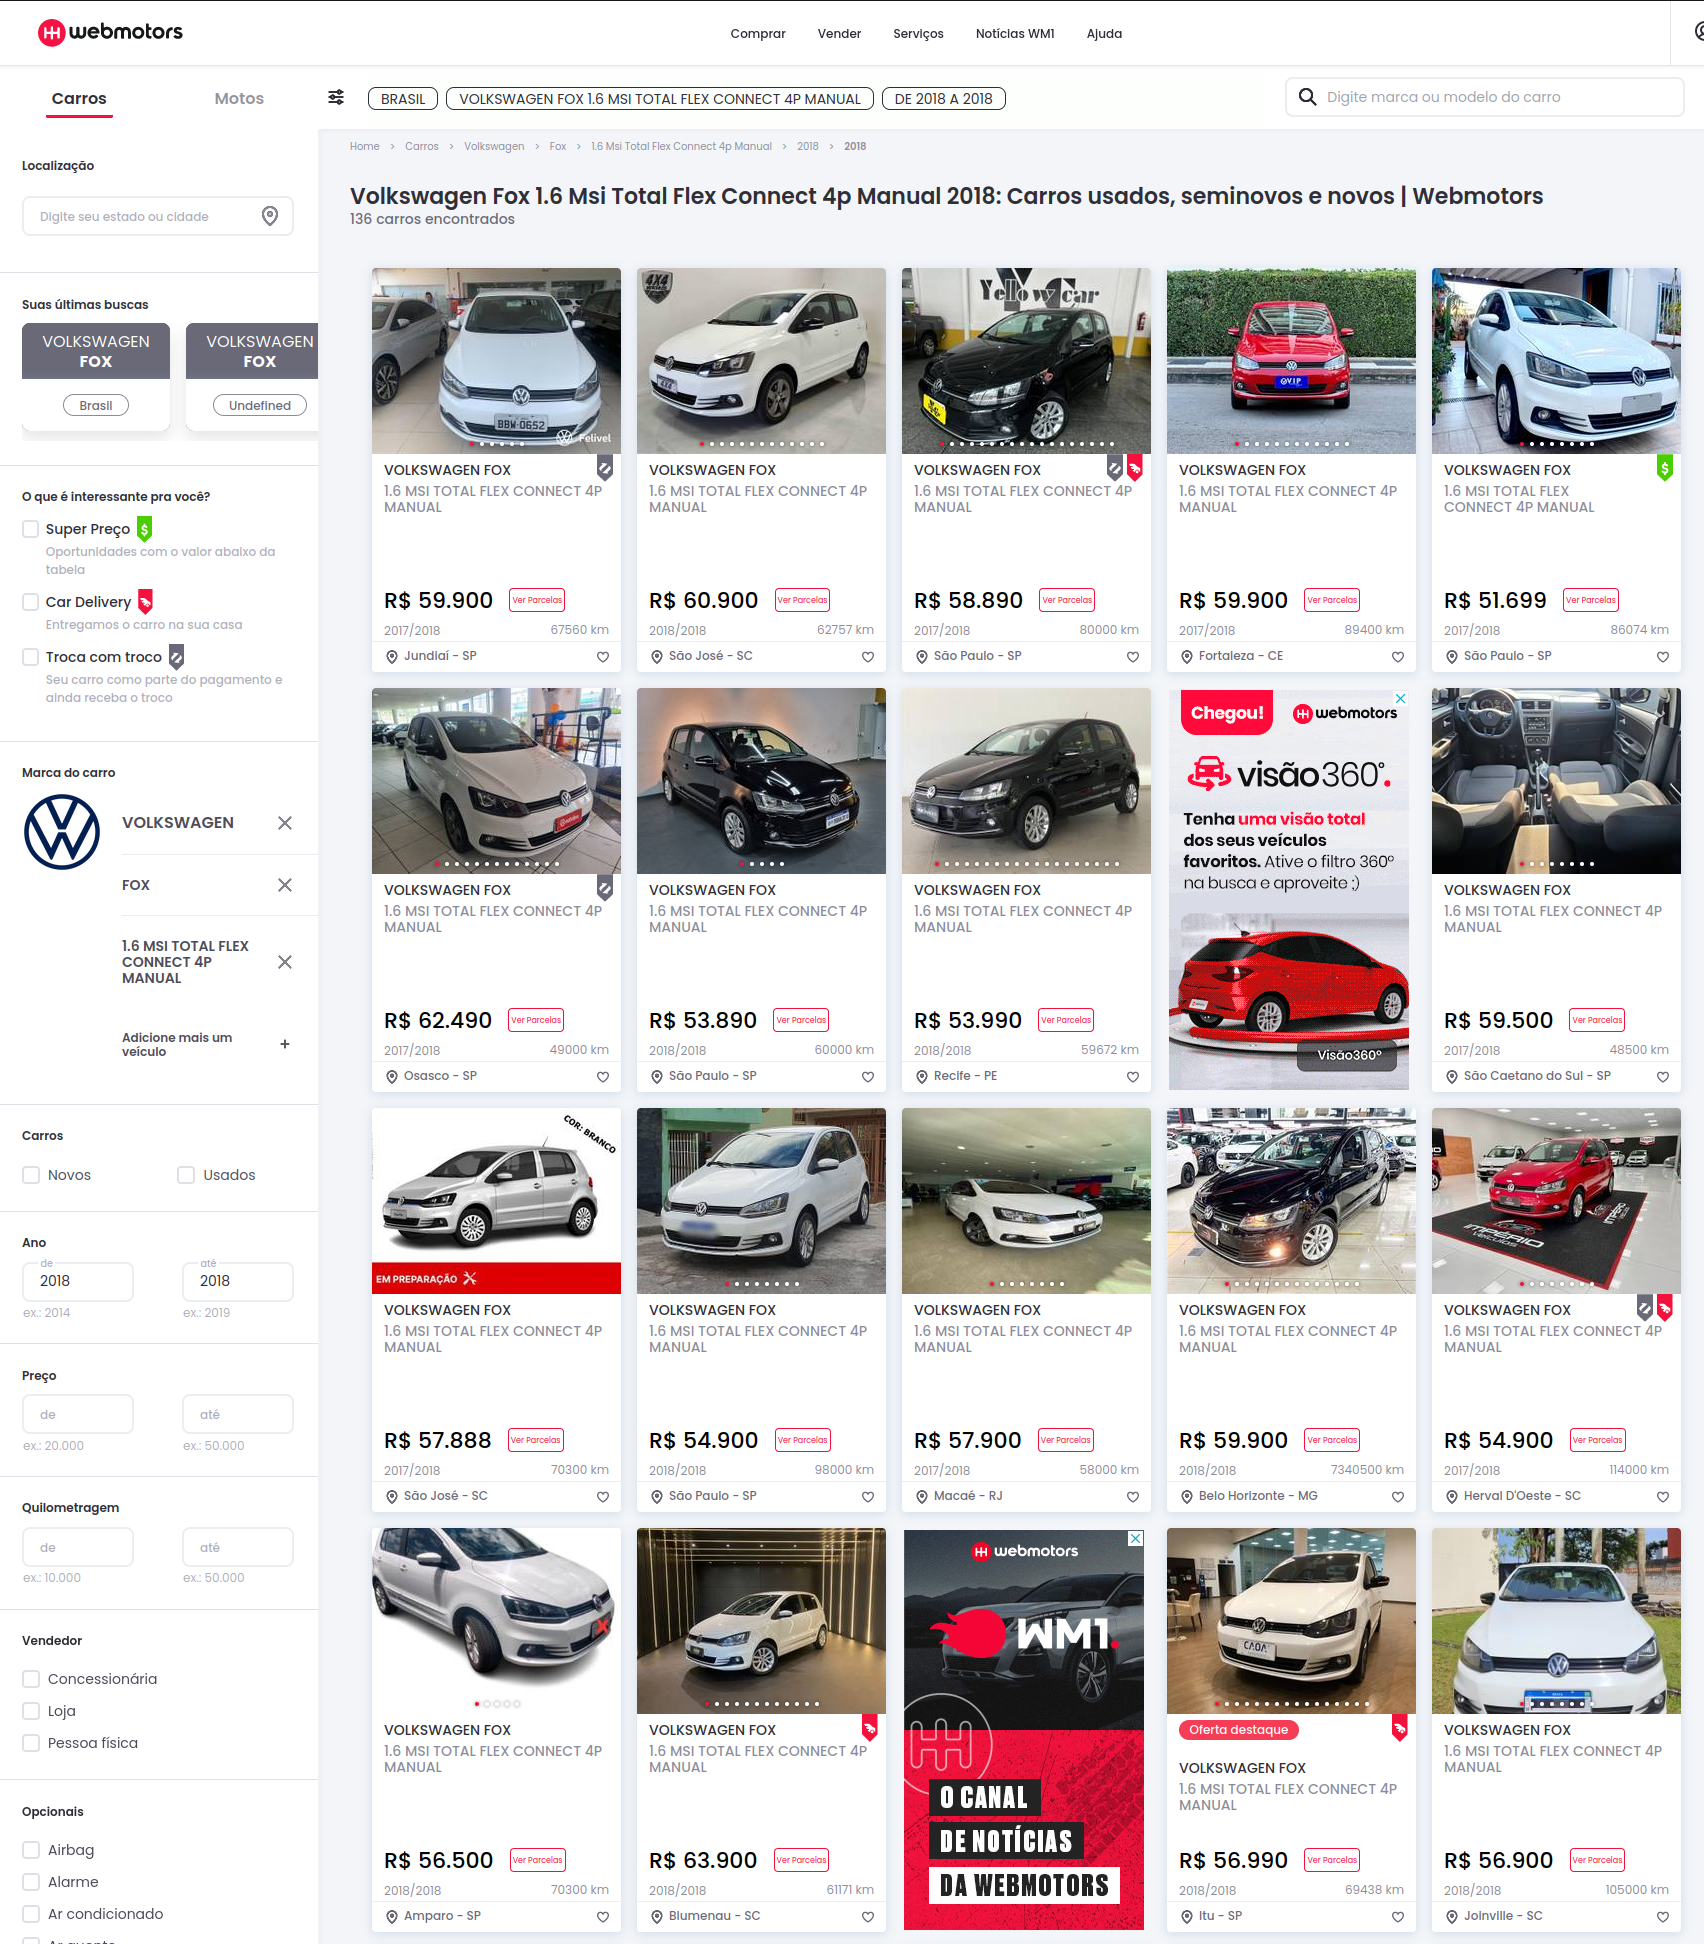
\includegraphics[width=250pt]{assets/webmotors.png}}
	\caption{Site de anúncios da WebMotors.}
	\label{fig5}
\end{figure}

Por definição, os anúncios são exibidos em ordem de "relevância" (conceito definido pela empresa - WebMotors ou OLX). Uma vez acessadas essas URLs, captura-se os campos HTML reverentes aos preços de até 20 anúncios na ordem de exibição.

Computa-se então, 3 valores (Mínimo, Médio e Máximo) para cada um dos portais, para o veículo correspondente.

\subsection{Indicadores Econômicos}

A coleta dos indicadores econômicos é realizada por um arquivo '.csv´ com colunas: Ano, Mês, IPC Geral, IGPM e IPCA.
 
Um script Python processa o arquivo e armazena no banco de dados.

O arquivo ".csv" é produzidos manualmente, em planilhas eletrônicas, com base nas informações acessadas nas páginas citadas como fonte de dados.

\section{Processamento e Armazenamento}

Os dados são processados e estruturados em um banco de dados relacional. Os próprios \textit{scripts} de carga realizam a organização dos dados e a distribuição nas tabelas.


\begin{figure}[htbp]
	\centerline{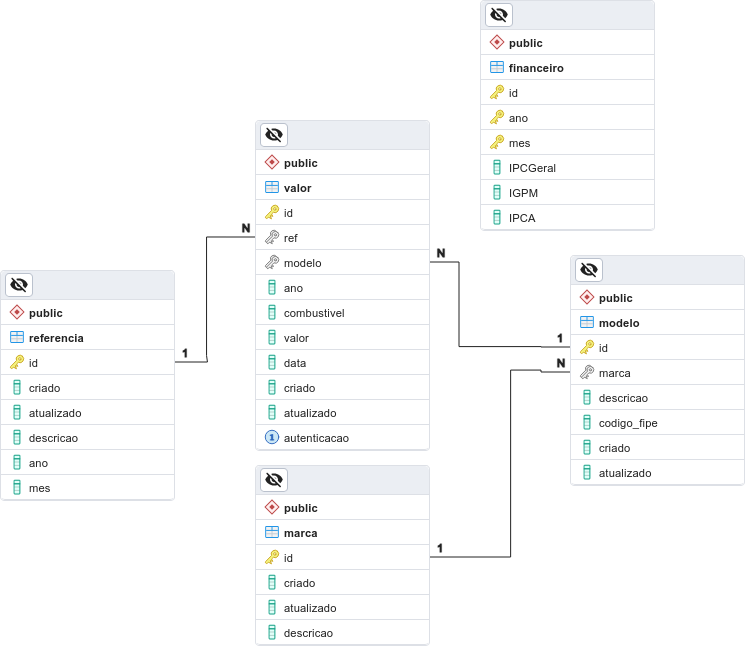
\includegraphics[width=250pt]{assets/database.png}}
	\caption{Modelo Entidade Relacionamento.}
	\label{fig1}
\end{figure}

Tabelas auxiliares para otimizar a geração dos gráficos são produzidas por \textit{scripts} periódicos com os dados de variação percentual do preço entre por referência (mês/ano) e modelo (código Fipe).

\section{Gerenciamento e Análise}

Para veículos com mais de 3 anos de uso, a solução realiza a previsão dos valores para 6 meses futuros, fornecendo ao usuário uma perspectiva para compra e venda.

Essa previsão é realizada com uma regressão utilizando um algoritmo KNN (\textit{K-Nearest Neighbors}) com k=3, atingindo um coeficiente de determinação (R\textsuperscript{2}) igual a 98,83%.


\begin{figure}[htbp]
	\centerline{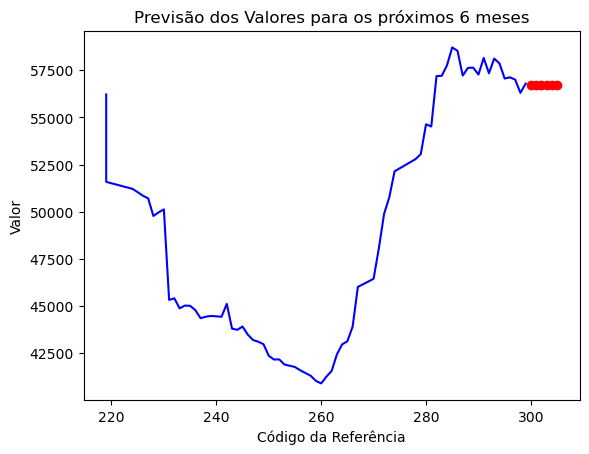
\includegraphics[width=250pt]{assets/previsao.png}}
	\caption{Gráfico da predição de 6 meses do preço.}
	\label{fig2}
\end{figure}


\section{Visualização e Interpretação}

Selecionado uma marca, um modelo e o ano de fabricação do veículo, a solução disponibiliza um \textit{`dashboard'} com o valor atual do veículo (segundo a Fipe), os valores mínimos, médios e máximos segundo o WebMotors e OLX e os gráficos:

\begin{itemize}
	\item série temporal do valor do ano de fabricação até o mês atual;
	
	\begin{figure}[h!]
		\centerline{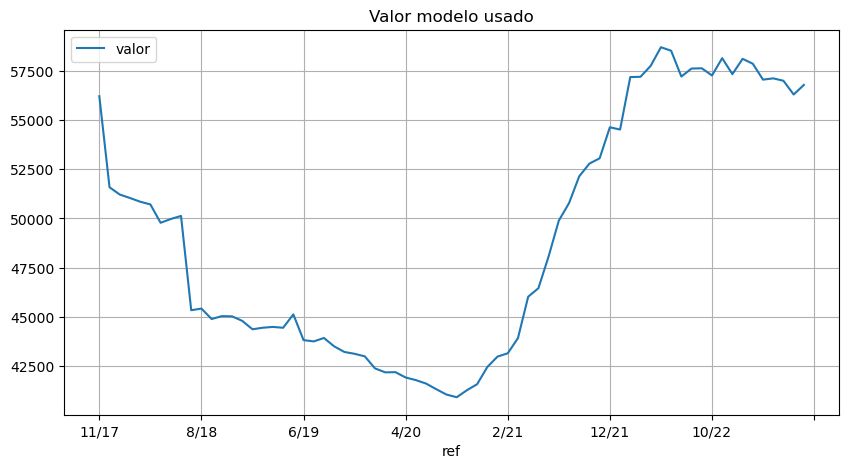
\includegraphics[width=250pt]{assets/precoUsado.png}}
		\caption{Preço do veículo usado.}
		\label{fig3}
	\end{figure}

	\item série temporal do valor `zero quilômetro' do ano de fabricação até o mês em que era disponível o modelo novo;
	
	
	\begin{figure}[h!]
		\centerline{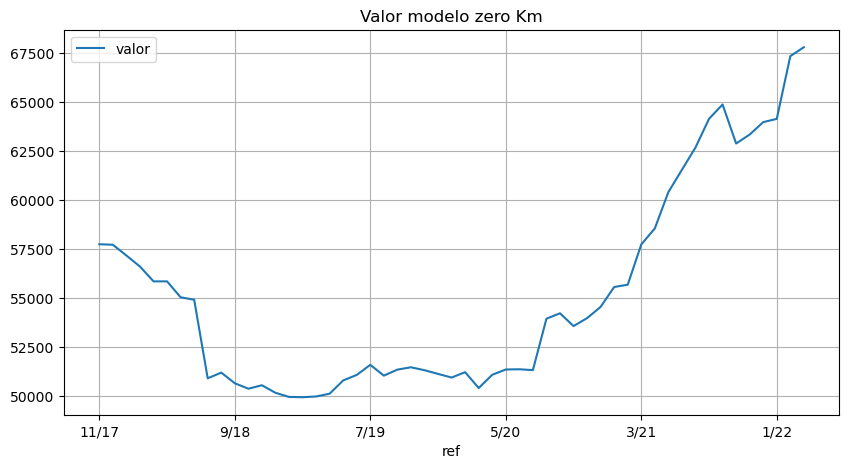
\includegraphics[width=250pt]{assets/precoZero.png}}
		\caption{Preço do veículo novo.}
		\label{fig4}
	\end{figure}
	
	
	\item série temporal demonstrando a variação percentual do valor do ano de fabricação até o mês atual junto com as curvas dos índices econômicos no mesmo período;
	
	
	\begin{figure}[h!]
		\centerline{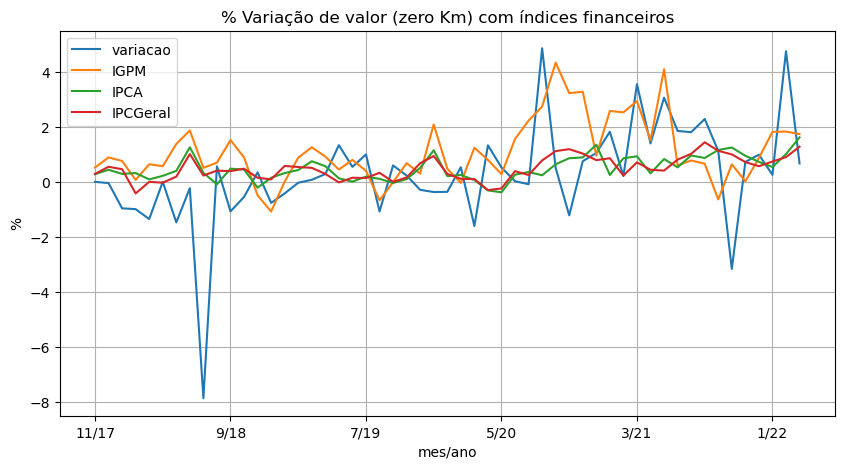
\includegraphics[width=250pt]{assets/varZero.png}}
		\caption{Variação do preço do veículo novo em comparação com índices financeiros.}
		\label{fig5}
	\end{figure}
	
	
	\item série temporal da variação percentual do valor do veículo `zero quilômetro' junto com as curvas dos índices econômicos no mesmo período.
	
	
	\begin{figure}[h!]
		\centerline{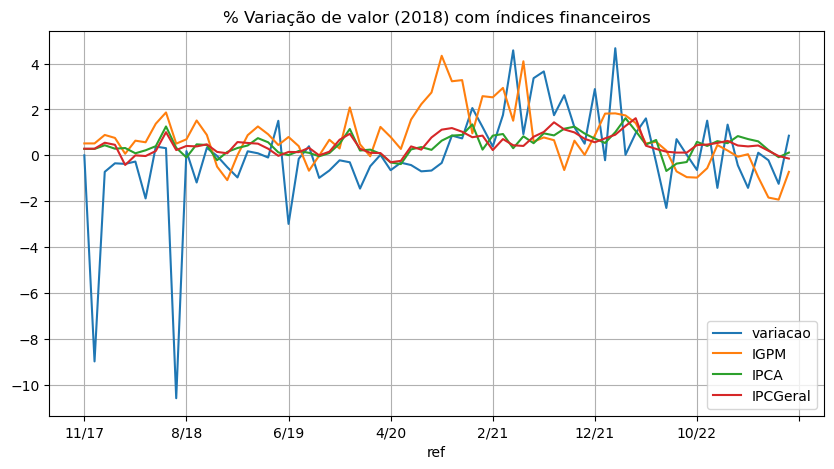
\includegraphics[width=250pt]{assets/varUsado.png}}
		\caption{Variação do preço do veículo usado em comparação com índices financeiros.}
		\label{fig6}
	\end{figure}
	
\end{itemize}

Os exemplos de gráficos utilizados referem-se ao veículo Modelo de código Fipe 005481-0 - `Fox Connect 1.6 Flex 8V 5p'.

É disponibilizado no \textit{`dashboard'}, também, os valores previstos para os próximos 6 meses pelo algoritmo.

Todos os arquivos fontes utilizados para elaboração deste artigo estão disponíveis em https://github.com/apcarneiro/autostats\_artigo.

\section{Conclusão}

O ensaio realizado para o protótipo demonstra que as informações sobre o mesmo veículo zero e usado são úteis para potencializar uma análise da desvalorização do veículo com o passar do tempo e auxiliar na tomada de decisão de compra/venda.

Ainda sobre os veículos usados, a comparação entre os valores de referência Fipe e os valores disponíveis nos anúncios dos `marketplaces' demonstram que os valores praticados pelo mercado variam em +/-15\% do referência Fipe (nas amostras exercitadas no ensaio - somente linha Volkswagen)

Já a comparação com os indicadores financeiros não parecem de grande ajuda, não impactando na variação do preço do carro zero quilômetro ou no carro usado.

De qualquer forma, parece ser uma boa fonte de apoio ao consumidor/vendedor para tomada de decisão sem que esse precise consultar muitas fontes.
 
Durante a pesquisa para esse ensaio, encontrou-se um portal que fornece parte das informações propostas em https://usados.umluizlima.dev. Porém as informações fornecidas são bem mais restritas e compreendem apenas 2 anos de `vida' do veículo.


\begin{thebibliography}{00}
	\bibitem{Fipe} Fipe - Fundação Instituto de Pesquisas Econômicas. https://www.fipe.org.br.
	\bibitem{Debit} Debit - https://debit.com.br.
	\bibitem{FGV} Fundação Getúlio Vargas - Índice Geral de Preços - Mercado https://portal.fgv.br/noticias/igp-m-resultados-2023
	\bibitem{IBGE} IBGE- Instituto Brasileiro de Geografia e Estatística - IPCA - Índice Nacional de Preços ao Consumidor Amplo https://www.ibge.gov.br/estatisticas/economicas/precos-e-custos/9256-indice-nacional-de-precos-ao-consumidor-amplo.html
\end{thebibliography}
\end{document}
